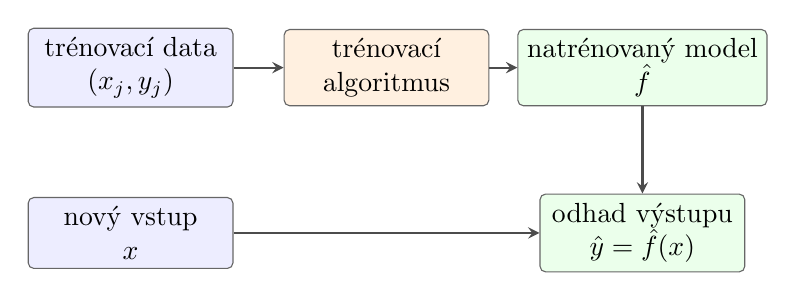
\begin{tikzpicture}[
    >=stealth,
    box/.style={
        draw=black!60,
        rounded corners=2pt,
        minimum width=2.6cm,
        minimum height=0.78cm,
        align=center
    },
    arr/.style={->, thick, draw=black!70}
]
    \node[box, fill=blue!7] (train) at (0,1.05)
        {trénovací data\\$(x_j,y_j)$};

    \node[box, fill=orange!12] (algorithm) at (3.25,1.05)
        {trénovací\\algoritmus};

    \node[box, fill=green!8] (model) at (6.5,1.05)
        {natrénovaný model\\$\hat f$};

    \node[box, fill=blue!7] (new) at (0,-1.05)
        {nový vstup\\$x$};

    \node[box, fill=green!8] (prediction) at (6.5,-1.05)
        {odhad výstupu\\$\hat y=\hat f(x)$};

    \draw[arr] (train) -- (algorithm);
    \draw[arr] (algorithm) -- (model);
    \draw[arr] (new) -- (prediction);
    \draw[arr] (model) -- (prediction);
\end{tikzpicture}
